\documentclass[11pt]{article}
\usepackage[T1]{fontenc}
\usepackage[margin=1in]{geometry}
\usepackage{amsmath,amssymb,amsthm,mathtools}
\usepackage{graphicx}
\usepackage{microtype}
\usepackage{xcolor}
\usepackage[colorlinks=true,linkcolor=blue!60!black,urlcolor=blue!70!black,citecolor=blue!60!black]{hyperref}

\newtheorem{theorem}{Theorem}
\newtheorem{lemma}[theorem]{Lemma}
\newtheorem{corollary}[theorem]{Corollary}
\newcommand{\SO}{\mathrm{SO}}
\newcommand{\OO}{\mathrm O}

\title{A weighted-cycle obstruction to a conjectured\\surjectivity from the orthogonal group}
\author{Candidate counterexample to the conjecture in arXiv:2408.04346}
\date{11 August 2026}

\begin{document}
\maketitle

\noindent
\fbox{\begin{minipage}{0.94\textwidth}
\textbf{Status: candidate counterexample, likely valid.}
For
\[
 \Phi_n(O)_{ij}^2=\frac12\bigl(O_{ij}^2+O_{ji}^2\bigr),
 \qquad O\in\SO(n),
\]
the source conjectures surjectivity onto the symmetric nonnegative matrices
whose Hadamard square is doubly stochastic. This is false already for
\(n=6\). A doubly stochastic matrix supported on a 6-cycle with alternating
edge weights \(1/3,2/3\) cannot be the symmetrized entrywise square of any
orthogonal matrix. The same construction disproves surjectivity for every
\(n\ge6\).
\end{minipage}}

\section{The source conjecture}

The source defines a weight matrix \(\Theta=\Phi_n(O)\) from a special
orthogonal matrix by
\[
 \Theta_{ij}=\sqrt{\frac12\bigl(O_{ij}^2+O_{ji}^2\bigr)}.
\]
It observes that \(\Theta\) is symmetric and that
\(P=\Theta\circ\Theta\) is doubly stochastic, then conjectures that this map
is surjective onto all symmetric nonnegative matrices having doubly
stochastic Hadamard square \cite[p.~5]{BGS}. The complete source page is
reproduced below.

\begin{center}
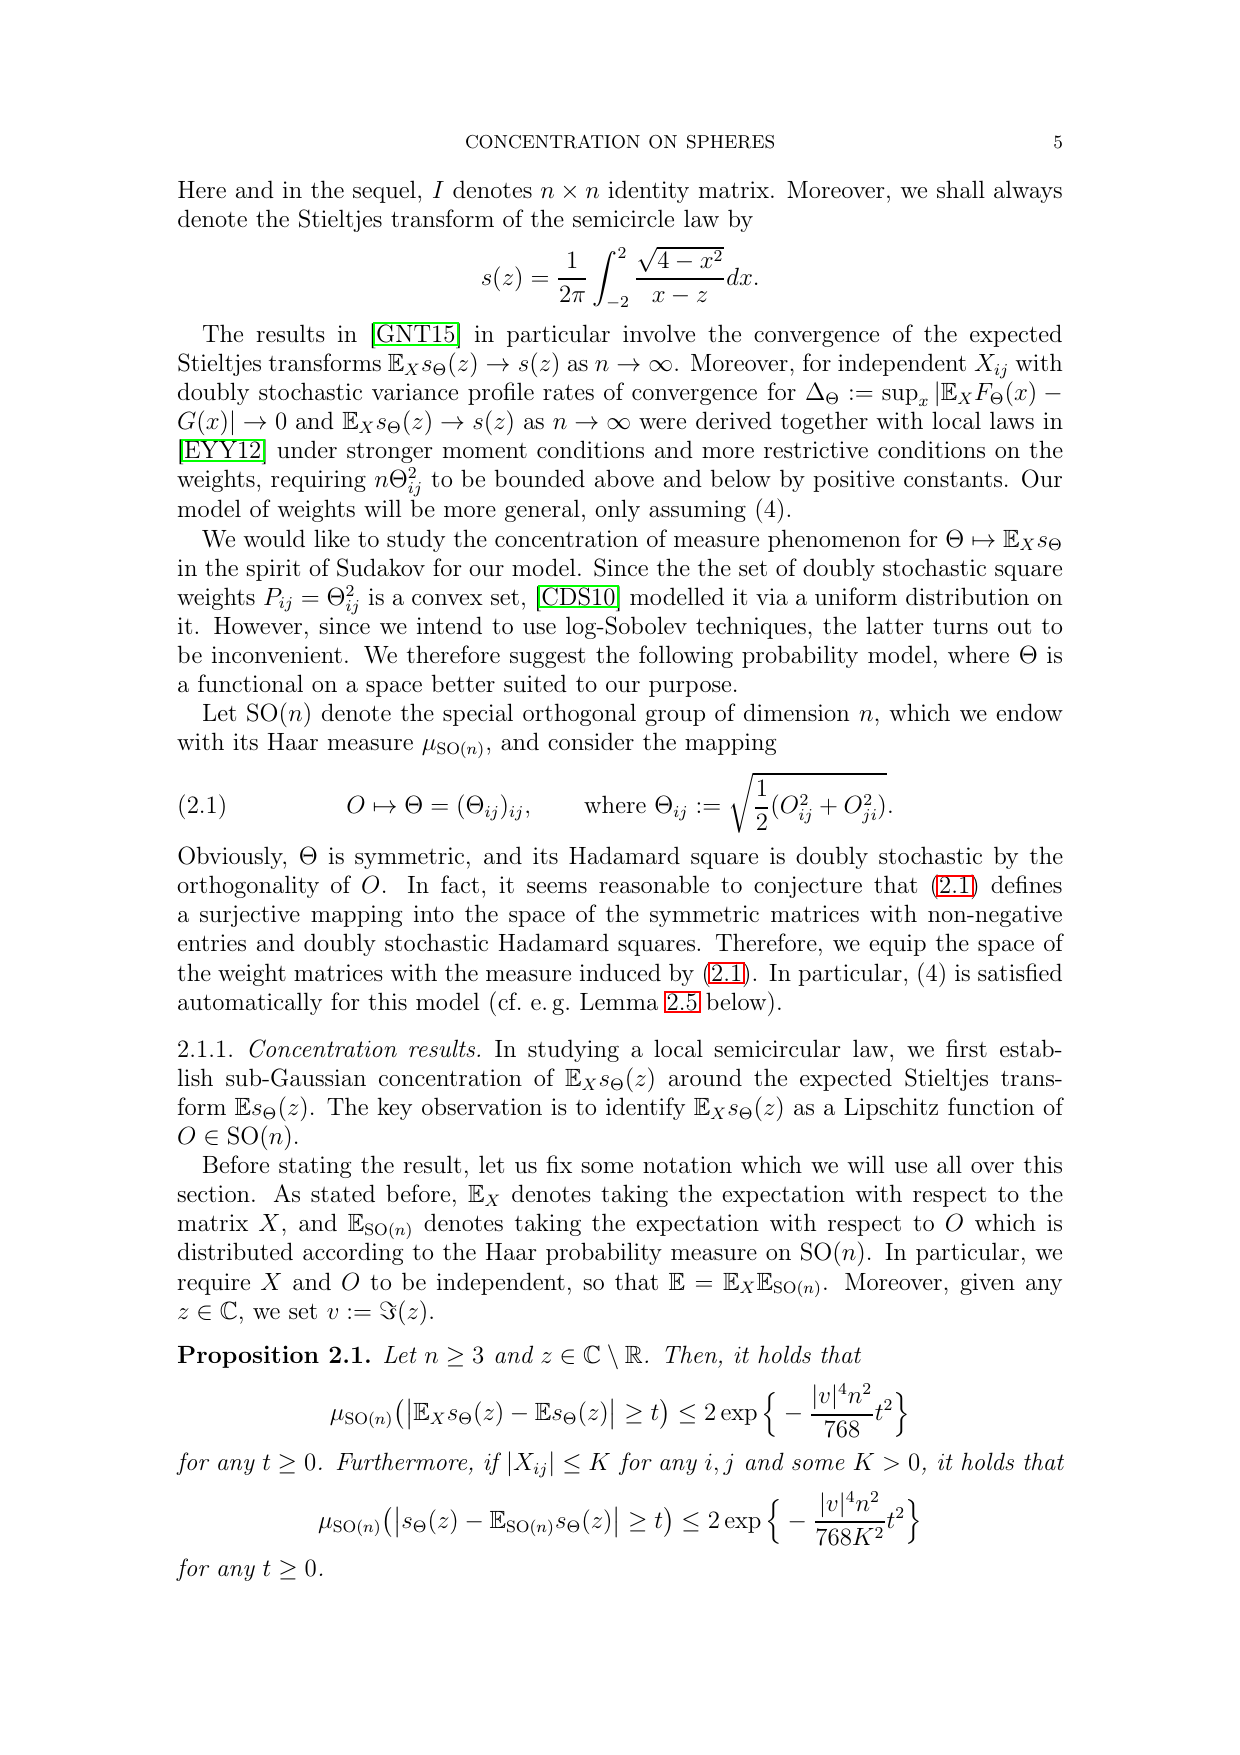
\includegraphics[height=0.72\textheight]{figures/source_candidate-05.png}
\end{center}

Equivalently, the conjecture says that every symmetric doubly stochastic
matrix \(P\) can be written
\begin{equation}\label{eq:map}
 P_{ij}=\frac12\bigl(O_{ij}^2+O_{ji}^2\bigr)
 \qquad(1\le i,j\le n)
\end{equation}
for some \(O\in\SO(n)\).

\section{Proof intuition}

Zeros in \(P\) are rigid: because the summands in \eqref{eq:map} are
nonnegative, \(P_{ij}=0\) forces both \(O_{ij}=0\) and \(O_{ji}=0\). We use a
sparse \(P\) whose support is an undirected cycle. On a cycle of length at
least five, two rows at distance two have only one possible common nonzero
column. Orthogonality forces one of those two entries to vanish. Column
normalization then forces the other to have modulus one. Repeating this
around the cycle makes \(O\) a signed permutation, whose symmetrized squared
entries can only be \(0\), \(1/2\), or \(1\). Fractional cycle weights such
as \(1/3\) and \(2/3\) are therefore impossible.

\section{Cycle-support rigidity}

Write indices modulo \(m\), and let \(C_m\) have edges
\(\{i,i+1\}\).

\begin{lemma}\label{lem:cycle}
Let \(m\ge5\). If \(O\in\OO(m)\) satisfies
\[
 O_{ij}=0
 \quad\text{whenever}\quad
 \{i,j\}\notin E(C_m),
\]
including \(O_{ii}=0\), then \(O\) is a signed permutation matrix.
\end{lemma}

\begin{proof}
Fix a column \(j\). Its only potentially nonzero entries are
\(O_{j-1,j}\) and \(O_{j+1,j}\). Rows \(j-1\) and \(j+1\) are supported,
respectively, in
\[
 \{j-2,j\}
 \qquad\text{and}\qquad
 \{j,j+2\}.
\]
Since \(m\ge5\), these two supports meet only in column \(j\).
Orthogonality of the two rows therefore gives
\[
 O_{j-1,j}O_{j+1,j}=0.
\]
On the other hand, column \(j\) has norm one, so
\[
 O_{j-1,j}^2+O_{j+1,j}^2=1.
\]
Exactly one entry in the column is thus \(\pm1\), and the other is zero.
This holds for every column. Orthogonality (or row normalization) then gives
exactly one \(\pm1\) in every row as well.
\end{proof}

\section{The counterexample}

\begin{theorem}\label{thm:main}
The map \(\Phi_6:\SO(6)\to\mathbb R^{6\times6}\) in the source is not
surjective onto the symmetric nonnegative matrices whose Hadamard squares
are doubly stochastic. In fact, the target matrix \(\Theta=P^{\circ1/2}\)
with
\[
P=\frac13
\begin{pmatrix}
0&1&0&0&0&2\\
1&0&2&0&0&0\\
0&2&0&1&0&0\\
0&0&1&0&2&0\\
0&0&0&2&0&1\\
2&0&0&0&1&0
\end{pmatrix}
\]
has no preimage even in \(\OO(6)\).
\end{theorem}

\begin{proof}
The matrix \(P\) is symmetric and nonnegative. Every row contains one entry
\(1/3\) and one entry \(2/3\), so every row and column sums to one. Thus
\(\Theta=P^{\circ1/2}\) belongs to the conjectured target.

Suppose \eqref{eq:map} held for an orthogonal \(O\). Whenever \(P_{ij}=0\),
nonnegativity in \eqref{eq:map} forces \(O_{ij}=O_{ji}=0\). Hence \(O\) is
supported on the displayed 6-cycle and has zero diagonal. By
Lemma~\ref{lem:cycle}, \(O\) is a signed permutation matrix. Therefore
\((O_{ij}^2,O_{ji}^2)\in\{0,1\}^2\), and \eqref{eq:map} forces
\[
 P_{ij}\in\{0,\tfrac12,1\}
 \qquad\text{for all }i,j.
\]
But every nonzero entry displayed in \(P\) is \(1/3\) or \(2/3\), a
contradiction.
\end{proof}

\begin{corollary}\label{cor:family}
For every even \(m\ge6\), alternating edge weights \(a,1-a\) on \(C_m\),
with
\[
 0<a<1,
 \qquad
 a\notin\{\tfrac12\},
\]
give a one-parameter family of counterexamples. Surjectivity also fails in
every dimension \(n\ge6\).
\end{corollary}

\begin{proof}
On an even cycle the alternating weights make every row sum one.
Lemma~\ref{lem:cycle} again forces any putative preimage to be a signed
permutation, while its symmetrized square has entries only in
\(\{0,1/2,1\}\). Since both \(a\) and \(1-a\) lie strictly between zero and
one and differ from \(1/2\), no preimage exists.

For arbitrary \(n\ge6\), take the direct sum of the displayed \(6\times6\)
matrix with \(I_{n-6}\). It is symmetric doubly stochastic. The zero
off-block entries would force any preimage to preserve the two blocks,
leaving the impossible 6-dimensional block.
\end{proof}

\section{Checks, upgrade attempts, and scope}

\paragraph{Independent finite check.}
Exact rational arithmetic verifies symmetry, nonnegativity, and all row sums
of \(P\). Enumerating the permutation matrices supported on \(C_6\) finds
four; every symmetrized square has entries in
\(\{0,1/2,1\}\), and none equals \(P\). The packet-local script
\texttt{code/verify\_weighted\_cycle.py} is confirmatory; the proof above is
exact and does not rely on enumeration.

\paragraph{Deep upgrades.}
The first construction targeted only \(n=6\). The support argument upgrades
it to a rigidity lemma for every cycle of length at least five, a
one-parameter counterexample family in every even dimension at least six,
and, by block embedding, failure in every dimension \(n\ge6\). The proof
does not determine whether surjectivity holds for \(n=3,4,5\); those smaller
cases are outside the counterexample claim.

\paragraph{Novelty check.}
Bounded primary-source searches through 11 August 2026 covered the exact
formula, the source title, symmetrized orthostochastic matrices, and
symmetric bistochastic matrices. They recovered the source and nearby work
on orthostochastic and symmetric-bistochastic subclasses, but no later
primary source stating this counterexample or resolving the conjecture. The
search was bounded, so novelty confidence is moderate.

\paragraph{Human-review recommendation.}
Check the zero-propagation step, the one-column intersection in
Lemma~\ref{lem:cycle}, and the direct-sum extension.

\begin{thebibliography}{9}
\bibitem{BGS}
F. G\"otze and H. Sambale,
\emph{Concentration of measure on spheres and related manifolds},
\href{https://arxiv.org/abs/2408.04346}{arXiv:2408.04346}.
\end{thebibliography}

\end{document}
